% Created by tikzDevice version 0.12.3.1 on 2021-04-09 17:45:03
% !TEX encoding = UTF-8 Unicode
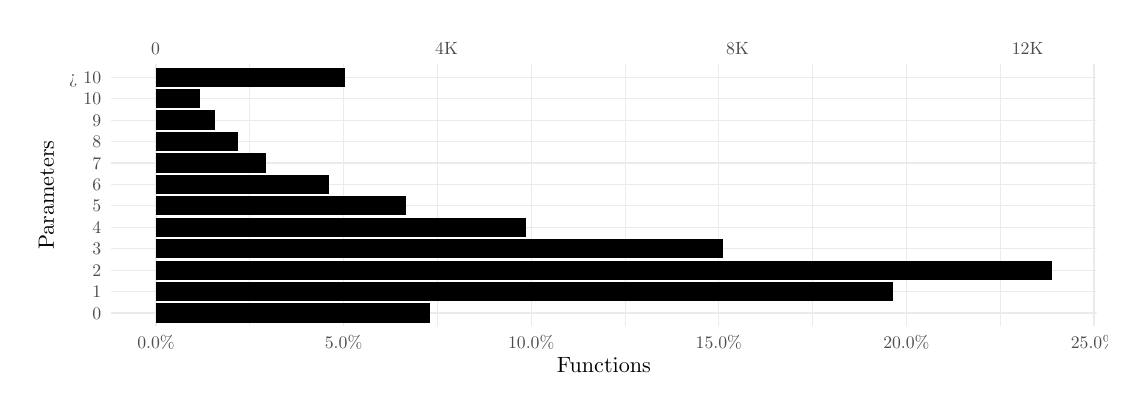
\begin{tikzpicture}[x=1pt,y=1pt]
\definecolor{fillColor}{RGB}{255,255,255}
\path[use as bounding box,fill=fillColor,fill opacity=0.00] (0,0) rectangle (390.26,130.09);
\begin{scope}
\path[clip] ( 30.17, 22.32) rectangle (386.26,116.83);
\definecolor{drawColor}{gray}{0.92}

\path[draw=drawColor,line width= 0.2pt,line join=round] ( 80.25, 22.32) --
	( 80.25,116.83);

\path[draw=drawColor,line width= 0.2pt,line join=round] (148.04, 22.32) --
	(148.04,116.83);

\path[draw=drawColor,line width= 0.2pt,line join=round] (215.84, 22.32) --
	(215.84,116.83);

\path[draw=drawColor,line width= 0.2pt,line join=round] (283.63, 22.32) --
	(283.63,116.83);

\path[draw=drawColor,line width= 0.2pt,line join=round] (351.42, 22.32) --
	(351.42,116.83);

\path[draw=drawColor,line width= 0.4pt,line join=round] ( 30.17, 26.97) --
	(386.26, 26.97);

\path[draw=drawColor,line width= 0.4pt,line join=round] ( 30.17, 34.71) --
	(386.26, 34.71);

\path[draw=drawColor,line width= 0.4pt,line join=round] ( 30.17, 42.46) --
	(386.26, 42.46);

\path[draw=drawColor,line width= 0.4pt,line join=round] ( 30.17, 50.21) --
	(386.26, 50.21);

\path[draw=drawColor,line width= 0.4pt,line join=round] ( 30.17, 57.95) --
	(386.26, 57.95);

\path[draw=drawColor,line width= 0.4pt,line join=round] ( 30.17, 65.70) --
	(386.26, 65.70);

\path[draw=drawColor,line width= 0.4pt,line join=round] ( 30.17, 73.45) --
	(386.26, 73.45);

\path[draw=drawColor,line width= 0.4pt,line join=round] ( 30.17, 81.20) --
	(386.26, 81.20);

\path[draw=drawColor,line width= 0.4pt,line join=round] ( 30.17, 88.94) --
	(386.26, 88.94);

\path[draw=drawColor,line width= 0.4pt,line join=round] ( 30.17, 96.69) --
	(386.26, 96.69);

\path[draw=drawColor,line width= 0.4pt,line join=round] ( 30.17,104.44) --
	(386.26,104.44);

\path[draw=drawColor,line width= 0.4pt,line join=round] ( 30.17,112.19) --
	(386.26,112.19);

\path[draw=drawColor,line width= 0.4pt,line join=round] ( 46.36, 22.32) --
	( 46.36,116.83);

\path[draw=drawColor,line width= 0.4pt,line join=round] (114.15, 22.32) --
	(114.15,116.83);

\path[draw=drawColor,line width= 0.4pt,line join=round] (181.94, 22.32) --
	(181.94,116.83);

\path[draw=drawColor,line width= 0.4pt,line join=round] (249.73, 22.32) --
	(249.73,116.83);

\path[draw=drawColor,line width= 0.4pt,line join=round] (317.52, 22.32) --
	(317.52,116.83);

\path[draw=drawColor,line width= 0.4pt,line join=round] (385.31, 22.32) --
	(385.31,116.83);
\definecolor{fillColor}{RGB}{0,0,0}

\path[fill=fillColor] ( 46.36,108.70) rectangle (114.49,115.67);

\path[fill=fillColor] ( 46.36, 23.48) rectangle (145.55, 30.45);

\path[fill=fillColor] ( 46.36, 31.23) rectangle (312.71, 38.20);

\path[fill=fillColor] ( 46.36,100.95) rectangle ( 62.37,107.92);

\path[fill=fillColor] ( 46.36, 38.97) rectangle (370.07, 45.95);

\path[fill=fillColor] ( 46.36, 46.72) rectangle (251.38, 53.69);

\path[fill=fillColor] ( 46.36, 54.47) rectangle (179.99, 61.44);

\path[fill=fillColor] ( 46.36, 62.22) rectangle (136.86, 69.19);

\path[fill=fillColor] ( 46.36, 69.96) rectangle (108.79, 76.94);

\path[fill=fillColor] ( 46.36, 77.71) rectangle ( 86.16, 84.68);

\path[fill=fillColor] ( 46.36, 85.46) rectangle ( 76.18, 92.43);

\path[fill=fillColor] ( 46.36, 93.20) rectangle ( 67.57,100.18);
\end{scope}
\begin{scope}
\path[clip] (  0.00,  0.00) rectangle (390.26,130.09);
\definecolor{drawColor}{gray}{0.30}

\node[text=drawColor,anchor=base,inner sep=0pt, outer sep=0pt, scale=  0.64] at ( 46.21,120.43) {0};

\node[text=drawColor,anchor=base,inner sep=0pt, outer sep=0pt, scale=  0.64] at (151.36,120.43) {4K};

\node[text=drawColor,anchor=base,inner sep=0pt, outer sep=0pt, scale=  0.64] at (256.51,120.43) {8K};

\node[text=drawColor,anchor=base,inner sep=0pt, outer sep=0pt, scale=  0.64] at (361.31,120.43) {12K};
\end{scope}
\begin{scope}
\path[clip] (  0.00,  0.00) rectangle (390.26,130.09);
\definecolor{drawColor}{gray}{0.30}

\node[text=drawColor,anchor=base east,inner sep=0pt, outer sep=0pt, scale=  0.64] at ( 26.57, 24.76) {0};

\node[text=drawColor,anchor=base east,inner sep=0pt, outer sep=0pt, scale=  0.64] at ( 26.57, 32.51) {1};

\node[text=drawColor,anchor=base east,inner sep=0pt, outer sep=0pt, scale=  0.64] at ( 26.57, 40.26) {2};

\node[text=drawColor,anchor=base east,inner sep=0pt, outer sep=0pt, scale=  0.64] at ( 26.57, 48.00) {3};

\node[text=drawColor,anchor=base east,inner sep=0pt, outer sep=0pt, scale=  0.64] at ( 26.57, 55.75) {4};

\node[text=drawColor,anchor=base east,inner sep=0pt, outer sep=0pt, scale=  0.64] at ( 26.57, 63.50) {5};

\node[text=drawColor,anchor=base east,inner sep=0pt, outer sep=0pt, scale=  0.64] at ( 26.57, 71.25) {6};

\node[text=drawColor,anchor=base east,inner sep=0pt, outer sep=0pt, scale=  0.64] at ( 26.57, 78.99) {7};

\node[text=drawColor,anchor=base east,inner sep=0pt, outer sep=0pt, scale=  0.64] at ( 26.57, 86.74) {8};

\node[text=drawColor,anchor=base east,inner sep=0pt, outer sep=0pt, scale=  0.64] at ( 26.57, 94.49) {9};

\node[text=drawColor,anchor=base east,inner sep=0pt, outer sep=0pt, scale=  0.64] at ( 26.57,102.23) {10};

\node[text=drawColor,anchor=base east,inner sep=0pt, outer sep=0pt, scale=  0.64] at ( 26.57,109.98) {> 10};
\end{scope}
\begin{scope}
\path[clip] (  0.00,  0.00) rectangle (390.26,130.09);
\definecolor{drawColor}{gray}{0.30}

\node[text=drawColor,anchor=base,inner sep=0pt, outer sep=0pt, scale=  0.64] at ( 46.36, 14.31) {0.0{\%}};

\node[text=drawColor,anchor=base,inner sep=0pt, outer sep=0pt, scale=  0.64] at (114.15, 14.31) {5.0{\%}};

\node[text=drawColor,anchor=base,inner sep=0pt, outer sep=0pt, scale=  0.64] at (181.94, 14.31) {10.0{\%}};

\node[text=drawColor,anchor=base,inner sep=0pt, outer sep=0pt, scale=  0.64] at (249.73, 14.31) {15.0{\%}};

\node[text=drawColor,anchor=base,inner sep=0pt, outer sep=0pt, scale=  0.64] at (317.52, 14.31) {20.0{\%}};

\node[text=drawColor,anchor=base,inner sep=0pt, outer sep=0pt, scale=  0.64] at (385.31, 14.31) {25.0{\%}};
\end{scope}
\begin{scope}
\path[clip] (  0.00,  0.00) rectangle (390.26,130.09);
\definecolor{drawColor}{RGB}{0,0,0}

\node[text=drawColor,anchor=base,inner sep=0pt, outer sep=0pt, scale=  0.80] at (208.22,  5.56) {Functions};
\end{scope}
\begin{scope}
\path[clip] (  0.00,  0.00) rectangle (390.26,130.09);
\definecolor{drawColor}{RGB}{0,0,0}

\node[text=drawColor,rotate= 90.00,anchor=base,inner sep=0pt, outer sep=0pt, scale=  0.80] at (  9.51, 69.58) {Parameters};
\end{scope}
\end{tikzpicture}
